%% (Master) Thesis template
% Template version used: v1.4
%
% Largely adapted from Adrian Nievergelt's template for the ADPS
% (lecture notes) project.


%% We use the memoir class because it offers a many easy to use features.
\documentclass[11pt,a4paper,titlepage]{memoir}

%% Packages
%% ========

%% LaTeX Font encoding -- DO NOT CHANGE
\usepackage[OT1]{fontenc}

%% Babel provides support for languages.  'english' uses British
%% English hyphenation and text snippets like "Figure" and
%% "Theorem". Use the option 'ngerman' if your document is in German.
%% Use 'american' for American English.  Note that if you change this,
%% the next LaTeX run may show spurious errors.  Simply run it again.
%% If they persist, remove the .aux file and try again.
\usepackage[english]{babel}

%% Input encoding 'utf8'. In some cases you might need 'utf8x' for
%% extra symbols. Not all editors, especially on Windows, are UTF-8
%% capable, so you may want to use 'latin1' instead.
\usepackage[utf8]{inputenc}

%% This changes default fonts for both text and math mode to use Herman Zapfs
%% excellent Palatino font.  Do not change this.
\usepackage[sc]{mathpazo}

%% The AMS-LaTeX extensions for mathematical typesetting.  Do not
%% remove.
\usepackage{amsmath,amssymb,amsfonts,mathrsfs}

%% NTheorem is a reimplementation of the AMS Theorem package. This
%% will allow us to typeset theorems like examples, proofs and
%% similar.  Do not remove.
%% NOTE: Must be loaded AFTER amsmath, or the \qed placement will
%% break
\usepackage[amsmath,thmmarks]{ntheorem}

%% LaTeX' own graphics handling
\usepackage{graphicx}

%% We unfortunately need this for the Rules chapter.  Remove it
%% afterwards; or at least NEVER use its underlining features.
\usepackage{soul}

%% This allows you to add .pdf files. It is used to add the
%% declaration of originality.
\usepackage{pdfpages}

%% Some more packages that you may want to use.  Have a look at the
%% file, and consult the package docs for each.
%% See the TeXed file for more explanations

%% [OPT] Multi-rowed cells in tabulars
%\usepackage{multirow}

%% [REC] Intelligent cross reference package. This allows for nice
%% combined references that include the reference and a hint to where
%% to look for it.
\usepackage{varioref}

%% [OPT] Easily changeable quotes with \enquote{Text}
%\usepackage[german=swiss]{csquotes}

%% [REC] Format dates and time depending on locale
\usepackage{datetime}

%% [OPT] Provides a \cancel{} command to stroke through mathematics.
%\usepackage{cancel}

%% [NEED] This allows for additional typesetting tools in mathmode.
%% See its excellent documentation.
\usepackage{mathtools}

%% [ADV] Conditional commands
%\usepackage{ifthen}

%% [OPT] Manual large braces or other delimiters.
%\usepackage{bigdelim, bigstrut}

%% [REC] Alternate vector arrows. Use the command \vv{} to get scaled
%% vector arrows.
\usepackage[h]{esvect}

%% [NEED] Some extensions to tabulars and array environments.
\usepackage{array}

%% [OPT] Postscript support via pstricks graphics package. Very
%% diverse applications.
%\usepackage{pstricks,pst-all}

%% [?] This seems to allow us to define some additional counters.
%\usepackage{etex}

%% [ADV] XY-Pic to typeset some matrix-style graphics
%\usepackage[all]{xy}

%% [OPT] This is needed to generate an index at the end of the
%% document.
%\usepackage{makeidx}

%% [OPT] Fancy package for source code listings.  The template text
%% needs it for some LaTeX snippets; remove/adapt the \lstset when you
%% remove the template content.
\usepackage{listings}
\lstset{language=TeX,basicstyle={\normalfont\ttfamily}}

%% [REC] Fancy character protrusion.  Must be loaded after all fonts.
\usepackage{microtype}

%% [REC] Nicer tables.  Read the excellent documentation.
\usepackage{booktabs}


%% Our layout configuration.  DO NOT CHANGE.
%% Memoir layout setup

%% NOTE: You are strongly advised not to change any of them unless you
%% know what you are doing.  These settings strongly interact in the
%% final look of the document.

% Dependencies
\usepackage{ETHlogo}

% Turn extra space before chapter headings off.
\setlength{\beforechapskip}{0pt}

\nonzeroparskip
\parindent=0pt
\defaultlists

% Chapter style redefinition
\makeatletter

\if@twoside
  \pagestyle{Ruled}
  \copypagestyle{chapter}{Ruled}
\else
  \pagestyle{ruled}
  \copypagestyle{chapter}{ruled}
\fi
\makeoddhead{chapter}{}{}{}
\makeevenhead{chapter}{}{}{}
\makeheadrule{chapter}{\textwidth}{0pt}
\copypagestyle{abstract}{empty}

\makechapterstyle{bianchimod}{%
  \chapterstyle{default}
  \renewcommand*{\chapnamefont}{\normalfont\Large\sffamily}
  \renewcommand*{\chapnumfont}{\normalfont\Large\sffamily}
  \renewcommand*{\printchaptername}{%
    \chapnamefont\centering\@chapapp}
  \renewcommand*{\printchapternum}{\chapnumfont {\thechapter}}
  \renewcommand*{\chaptitlefont}{\normalfont\huge\sffamily}
  \renewcommand*{\printchaptertitle}[1]{%
    \hrule\vskip\onelineskip \centering \chaptitlefont\textbf{\vphantom{gyM}##1}\par}
  \renewcommand*{\afterchaptertitle}{\vskip\onelineskip \hrule\vskip
    \afterchapskip}
  \renewcommand*{\printchapternonum}{%
    \vphantom{\chapnumfont {9}}\afterchapternum}}

% Use the newly defined style
\chapterstyle{bianchimod}

\setsecheadstyle{\Large\bfseries\sffamily}
\setsubsecheadstyle{\large\bfseries\sffamily}
\setsubsubsecheadstyle{\bfseries\sffamily}
\setparaheadstyle{\normalsize\bfseries\sffamily}
\setsubparaheadstyle{\normalsize\itshape\sffamily}
\setsubparaindent{0pt}

% Set captions to a more separated style for clearness
\captionnamefont{\sffamily\bfseries\footnotesize}
\captiontitlefont{\sffamily\footnotesize}
\setlength{\intextsep}{16pt}
\setlength{\belowcaptionskip}{1pt}

% Set section and TOC numbering depth to subsection
\setsecnumdepth{subsection}
\settocdepth{subsection}

%% Titlepage adjustments
\pretitle{\vspace{0pt plus 0.7fill}\begin{center}\HUGE\sffamily\bfseries}
\posttitle{\end{center}\par}
\preauthor{\par\begin{center}\let\and\\\Large\sffamily}
\postauthor{\end{center}}
\predate{\par\begin{center}\Large\sffamily}
\postdate{\end{center}}

\def\@advisors{}
\newcommand{\advisors}[1]{\def\@advisors{#1}}
\def\@department{}
\newcommand{\department}[1]{\def\@department{#1}}
\def\@thesistype{}
\newcommand{\thesistype}[1]{\def\@thesistype{#1}}

\renewcommand{\maketitlehooka}{\noindent\ETHlogo[2in]}

\renewcommand{\maketitlehookb}{\vspace{1in}%
  \par\begin{center}\Large\sffamily\@thesistype\end{center}}

\renewcommand{\maketitlehookd}{%
  \vfill\par
  \begin{flushright}
    \sffamily
    \@advisors\par
    \@department, ETH Z\"urich
  \end{flushright}
}

\checkandfixthelayout

\setlength{\droptitle}{-48pt}

\makeatother

% This defines how theorems should look. Best leave as is.
\theoremstyle{plain}
\setlength\theorempostskipamount{0pt}

%%% Local Variables:
%%% mode: latex
%%% TeX-master: "thesis"
%%% End:


%% Theorem environments.  You will have to adapt this for a German
%% thesis.
%% Theorem-like environments

%% This can be changed according to language. You can comment out the ones you
%% don't need.

\numberwithin{equation}{chapter}

%% German theorems
%\newtheorem{satz}{Satz}[chapter]
%\newtheorem{beispiel}[satz]{Beispiel}
%\newtheorem{bemerkung}[satz]{Bemerkung}
%\newtheorem{korrolar}[satz]{Korrolar}
%\newtheorem{definition}[satz]{Definition}
%\newtheorem{lemma}[satz]{Lemma}
%\newtheorem{proposition}[satz]{Proposition}

%% English variants
\newtheorem{theorem}{Theorem}[chapter]
\newtheorem{example}[theorem]{Example}
\newtheorem{remark}[theorem]{Remark}
\newtheorem{corollary}[theorem]{Corollary}
\newtheorem{definition}[theorem]{Definition}
\newtheorem{lemma}[theorem]{Lemma}
\newtheorem{proposition}[theorem]{Proposition}

%% Proof environment with a small square as a "qed" symbol
\theoremstyle{nonumberplain}
\theorembodyfont{\normalfont}
\theoremsymbol{\ensuremath{\square}}
\newtheorem{proof}{Proof}
%\newtheorem{beweis}{Beweis}


%% Helpful macros.
%% Custom commands
%% ===============

%% Special characters for number sets, e.g. real or complex numbers.
\newcommand{\C}{\mathbb{C}}
\newcommand{\K}{\mathbb{K}}
\newcommand{\N}{\mathbb{N}}
\newcommand{\Q}{\mathbb{Q}}
\newcommand{\R}{\mathbb{R}}
\newcommand{\Z}{\mathbb{Z}}
\newcommand{\X}{\mathbb{X}}

%% Fixed/scaling delimiter examples (see mathtools documentation)
\DeclarePairedDelimiter\abs{\lvert}{\rvert}
\DeclarePairedDelimiter\norm{\lVert}{\rVert}

%% Use the alternative epsilon per default and define the old one as \oldepsilon
\let\oldepsilon\epsilon
\renewcommand{\epsilon}{\ensuremath\varepsilon}

%% Also set the alternate phi as default.
\let\oldphi\phi
\renewcommand{\phi}{\ensuremath{\varphi}}


%% Make document internal hyperlinks wherever possible. (TOC, references)
%% This MUST be loaded after varioref, which is loaded in 'extrapackages'
%% above.  We just load it last to be safe.
\usepackage[linkcolor=black,colorlinks=true,citecolor=black,filecolor=black]{hyperref}
\usepackage{listings}
\usepackage{xcolor}

% Define your code style
\lstset{
    language=Java,    % change this to your language
    basicstyle=\ttfamily\small,
    captionpos=b,
    keywordstyle=\color{blue},
    commentstyle=\color{green!60!black},
    stringstyle=\color{red},
    numbers=left,
    numberstyle=\tiny\color{gray},
    breaklines=false,
    showspaces=false,
    showstringspaces=false,
    tabsize=2
}
\newunicodechar{⟨}{\ensuremath{\langle}}
\newunicodechar{⟩}{\ensuremath{\rangle}}


%% Document information
%% ====================

\title{Verified Instruction Selection Pipeline in Lean4:
LLVM IR to ISA}
\author{S. Kuhn}
\thesistype{Bachelor Thesis}
\advisors{Advisors: }
\department{Department of Computer Science}
\date{March 05, 2025}

\begin{document}

\frontmatter

%% Title page is autogenerated from document information above.  DO
%% NOT CHANGE.
\begin{titlingpage}
  \calccentering{\unitlength}
  \begin{adjustwidth*}{\unitlength-24pt}{-\unitlength-24pt}
    \maketitle
  \end{adjustwidth*}
\end{titlingpage}

%% The abstract of your thesis.  Edit the file as needed.
\begin{abstract}
 Our implementation of a verified instruction selection pipeline from a subset of LLVM IR, produced by the Lean compiler, to ARM machine code is a first step toward strengthening trust in Lean’s translation process and proof by reflection, with the long-term goal of a fully verified Lean theorem proving infrastructure. The Lean interactive theorem prover plays a crucial role in formal verification. While its kernel has been verified, its compiler remains largely unverified. This is concerning for proof by reflection, where computations act as certificates for proofs, making compiler correctness essential for trustworthiness. We counteract this gap by implementing and verifying an instruction selection pass that translates LLVM IR to ARM assembly in Lean4 while preserving program semantics. We target a subset of LLVM IR commonly produced by the Lean compiler—load/store operations and integer arithmetic— and translate it to an ISA exhibiting formal correctness guarantees. Our implementation leverages formal models of LLVM and ARM and incorporates peephole optimization patterns for improved instruction selection. By utilizing bv\_ decide, a tactic within Lean allowing for automated bit vector reasoning, we gain significantly more proof automation compared to other projects like CompCert. The primary results of this work establish that any translation from LLVM IR to ARM machine code using our pipeline provides formal correctness guarantees proven in Lean.   
 
\end{abstract}


%% TOC with the proper setup, do not change.
\cleartorecto
\tableofcontents
\mainmatter

%% Your real content!
\chapter{Background}
In this chapter, we are going to prepare the reader with basic foundations to understand the work implemented by this thesis.
We are going to focus on the design of the LLVM compiler framework, its IR and its subproject, MLIR.
LLVM COMPILER TOOLCHAIN
(DIFFRENT STEPS AND PASSES AND ESPECIALLY CODE GENERATION)
THEN LLVM IR
THEN MLIR 
RISC-V
SEMANTICS AKA HOW THEY ARE DISPLAYED NOWDAYS
    LLVM IR SEMANTICS 
    RISCVV SEMANTIC (SAIL)

LEAN4 THEOREM PROVER 
    BASICS
    PROVING IN LEAN
    BV DECIDE AND LEANS BIT VECTOR LIBRARY

LEAN-MLIR FRAMEWORK (INTRODUCE IT VERY SIMPPLE AND GO IN MORE EPTH LATER )

\subchapter{The LLVM compiler ecosystem}
The LLVM project is an open-source collection of modular and reusable compiler components and toolchain technologies. It was started as a research project and gained in popularity such that it now is used as the compiler framework various programming languages. In this section we will the explain the compilation flow of LLVM and familiirze the reader with the its IR and the MLIR project within LLVM.

\subsubsection{LLVM compiler design}
Compilers are tools that translate a source program written in a high-level language into their machine code representation. Traditionally, compiler based on the LLVM project compromise the following stages:
\begin{enumerate}
  \item Lexing: Source code gets transformed into a token stream.
  \item Parsing: Converts the token stream into an abstract syntax tree (AST).
  \item Emit IR: AST to IR.
  \item IR-to-IR optimizations
  \item Code generation: IR to machine code lowering.
\end{enumerate}
LLVM itself is not a full compiler, but it provides the infrastructure for the last two stages of compilation stage. After providing a frontend that lowers to LLVM IR, any source langauge can leverage the optimization tools and code generation provided by LLVM. 

LLVM exhibtis its own intermediate representation which is used throught the entire LLVM toolchain. LLVM IR abstracts away source language specic features that would not allows to optimize in


LVM IR focuses on providing a language that is less abstract than a fully source level language but allows for enough of abstraction to employ optimizations that apply across various machine targets, unlikely assembley level optimizations.
a plattform indpenednt way but is still more high-level then assembly code where a lot of the semantics for opitmizations is hidden. 
LLVM IR is optimized in an iterative manner by applying diffrent analysis and optimization passes to its IR in an modular way. These passes are assumed to preserve code integrity and the semantics of the original source program. A pass within LLVM's transformation pass list is InstCombine,which applies peephole rewrites to programs in their LLVM IR form. A user can define which pass to apply by providing the corresponding flag to the LLVM optimizer via the command line or use the predefined set of optimization passes by LLVM by providing the optimization flags -01 to -O3.
Many programming langages provide a front-end, which compiles source code to LLVM IR and then leverages the LLVM backends.
LLVM code generator consists of three substages:
[insert code generation: legalization -> instruction selection -> instruction scheduling].
The modular design of LLVM allows the backend to be reused for any source language that compiles to the specific target architecture.


\textbf{LLVM and LLVM IR}
LLVM IR is a target-independent intermediate representation (IR) at the core of the LLVM (Low-Level Virtual Machine) compiler framework. LLVM is a open-source compiler infrastructure used in academia and industry. LLVM compilers typically lower source programs from high-level languages such as C, C++, Rust, or Haskell into LLVM IR. This intermediate form serves as a common, platform-independent abstraction over machine code to which source languages get lowered before  machine code is omited. Therefore LLVM IR acts as the central language throughout the LLVM compilation pipeline. Once a program is lowered into LLVM IR, a series of IR-to-IR transformations are applied. After these transformations, various LLVM backends further lower the optimized IR into machine code for a specific target architecture. By decoupling the optimization and backend phases from the source language, LLVM IR facilitates reuse and simplifies backend development. LLVM IR focuses on providing a language that is less abstract than a fully source level language but allows for enough of abstraction to employ optimizations that apply across various machine targets, unlikely assembley level optimizations. This abstraction makes LLVM IR suitable for implementing optimizations that are shared and reused across different source and target languages. Thus the implementation and verification of LLVM components, as well as components that interface with LLVM IR can be reused across a wide range of source languages that target LLVM.
\begin{figure}[htbp]
  \centering
  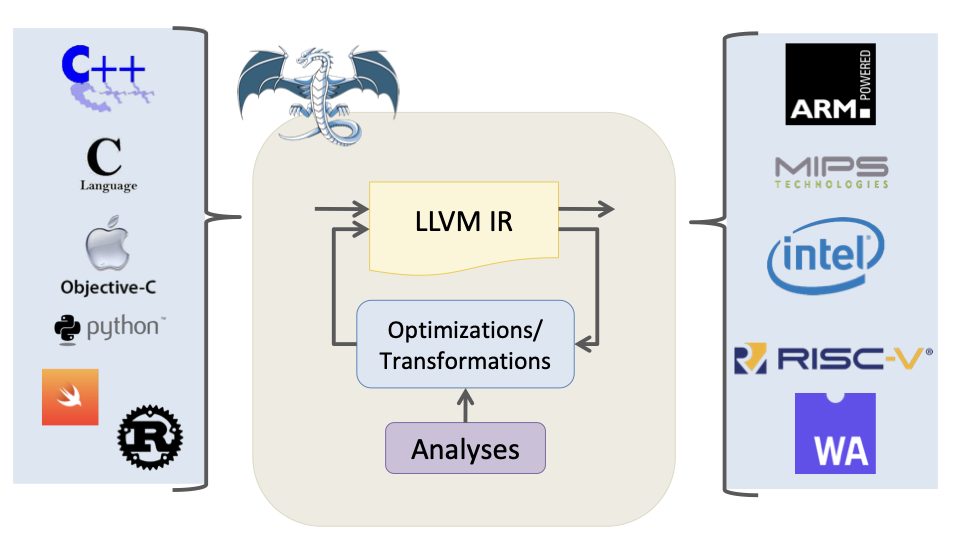
\includegraphics[scale=0.37]{thesis/llvm.png}
 
  \caption{LLVM compiler infrastrucutre with LLVM IR at its heart}
  \label{fig:your-label}
\end{figure}

LLVM IR is typed and in single static assignment form (SSA), which means that every variable has a type and is associated with only one specific definition point in the code. This allows for simplified compiler optimizations along def-use chains, as any use of a variable can be backtracked to a single place where the variable receives a value (def). 

[TO DO INSERT OVERVIEW OF LLVM IR ]

LLVM IR supports common types such as integers of different widths, as well as structured data. To handle non-initialized variables, LLVM IR supports an undef constant in its IR, which represents a set of possible values. When the LLVM compiler encounters an undef it is free to pick any convenient value of the correct type. Besides undef, LLVM IR  has poison values and undefined behaviour. All of these different notions of the future, where the compiler does not want to provide guarantees for a specific value or indicates a unsafe operation. This in turn makes the semantics of LLVM IR inherently non-deterministic and will be discussed in detail in section []. 
% Some commands used in this file
\newcommand{\package}{\emph}

\chapter{Introduction}
Lean [1,2] is a proof assistant and purely functional programming language, providing users with a tool for interactive theorem proving and software development. Lean itself offers a compiler that produces fast native code, which is written by translating Lean source code into Lean's core language, which will then be subsequently lowered to LLVM IR and then via the LLVM backend compiled into machine code specific for the target architecture [3]. As this compilation path leverages the optimizations and backend provided by LLVM to produce fast code, it heavily relies on the LLVM compiler toolchain. 

The Lean compiler is used not only to produce executables from Lean source code but is also crucial in a style of proof called 'proof by reflection' where a computation is executed, and the output of the computation is used as a certificate for a proof. This use of the compiler for proving makes verifying the Lean compiler an important research target, since the trustworthiness of fast proof by reflection in Lean hinges on the trustworthiness of its compiler toolchain. However, LLVM's large codebase with numerous optimization passes makes such a verification complex [4]. Full verification of Lean's compilation process is unlikely as it requires a fully verified LLVM compiler, while verification efforts for LLVM currently only cover its higher-level stacks around LLVM-IR (e.g., Vellvm [5]) and also only exist in ROCQ [6]. As a first step towards a verified Lean backend, with an eye towards providing trustworthy proof by reflection for Lean, this work proposes to develop a verified instruction selection pipeline that translates LLVM IR into an ISA, here choosen to be RISC-V, to produce fast machine-specific code. This verified instruction selection pipeline aims to provide formal guarantees that the RISC-V assembly code generated from Lean source programs stays semantically equivalent to the LLVM IR representation of the program in Lean’s core language. While the actual connection to Lean’s core language is a non-goal, we will focus in this project on the subset of LLVM-IR that would typically be generated by Lean, e.g., LLVM-IR consisting of load/store operations plus integer arithmetic.

To implement such a formally verified instruction selection pass, we leverage and build upon existing RISC-V and LLVM specifications and publically available datasets of peephole optimizations (e.g., from the GCC compiler backend). The Lean-MLIR project [7] already provides a semantic model of the arithmetic fragment of LLVM, which can be used as a starting point for the needed LLVM semantics. RISC-V semantics are also well-defined and given in a formal specification by the SAIL project1 [8]. Additionally, compiler backends like in GCC or LLVM provide a repository with an extensive collection of peephole optimization patterns, which we could adapt to an LLVM-like abstract ISA and leverage to write our verified instruction selection pipeline to generate optimized machine code.

We shall use the insights from projects like Peek [9], which implements a peephole optimization pass for x86 in CompCERT [10]. In this work, we will integrate the use of verification tools to formally show the semantic equivalence of the LLVM IR instructions to be lowered and our generated RISC-V lowering. Leveraging bv\underline decide [7], the first fully verified SMT solver natively integrated into an interactive theorem prover, we gain significantly more proof automation compared to other projects like CompCert. Therefore, we shall attempt to automate many of these proofs using SMT-LIB compatible proof automation ( bv \underline decide) and Lean’s extensive bit vector library.


\chapter{Background }

This chapter will give the background needed to understand the core work of this thesis. 

\section{Foundations of Automatic and Interactive Theorem Proving} 
-

\section{Lean4 Foundations} 
\subsection{Bit Vector Support in Lean: BitVec and bv\_decide} 
\textbf{Bit Vectors in Lean:}
Bitvectors are fixed-width binary sequences that provide a mathematical abstraction for modeling machine-level data representation. A bitvector of width $w$ formally represents an element from the set $\{0, 1, \ldots, 2^w - 1\}$, which corresponds to the possible values that can be stored in a $w$-bit register. This representation is foundational in formal verification of hardware designs, instruction set architectures, and low-level software systems like compilers where bit vectors e.g enable reasoning about register operations. The Lean theorem prover supports reasoning about finite bit vectors through the \textit{BitVec} type, which represents a natural number \textit{n} with a proof that \( n < 2^w \). Specifcally \textit{BitVec} is implemented as "a wrapper around \textit{Fin} with a suitable bound". In Lean, the type \textit{Fin n} represents the finite set of natural numbers strictly less than n. An element of type \textit{Fin n} consist of a natural number \textit{val}, and a proof that \textit{val \( < \) n}. Both \textit{Fin} and  \textit{BitVec} exemplify Lean's dependent typing capabilities, as their type definitions depend on a value (the upper bound n or width w, respectively). \textit{Fin} itself is built upon \textit{Nat} (natural numbers), which have strong support in Lean's kernel.


\begin{lstlisting} [language=Lean, caption= bit vector represenation in Lean]
structure Fin (n : Nat) where
  val : Nat
  isLt : val < n 
-- type Fin n represents the finite set of natural numbers
strictly less than n, including a proof that val < n.

def BitVec (w : Nat) := { n : Nat // n < 2^w }
-- type BitVec represents the finite set of natural numbers
val, including a proof that n < 2^w.
\end{lstlisting}

 The design choice of wrapping the implementation of \textit{BitVec} around \textit{Fin} and \textit{Nat} allows for efficient reasoning about bit vectors by leveraging Lean's optimized natural number operations while maintaining the formal constraint of boundedness through dependent typing.
In compiled code, the representations of \textit{Fin, BitVec}  and \textit{Nat} are indistinguishable and efficient, leaving only the underlying natural number representation.

\noindent
\begin{lstlisting} [language=Lean, caption= Example of defining a Fin in the range of 0 to 31 with value 19 in Lean]
def exampleFin : Fin 32  :=  <19 , by simp [Nat.reduceLT]>
\end{lstlisting}
\begin{lstlisting} [language=Lean, caption= Example of defining a BitVec of width 32 with value 42 in Lean]
def bv32_ex1 : BitVec 32 :=  
            <42, by simp [Nat.reducePow, Nat.reduceLT]>
def bv32_ex2 : BitVec 32 :=  42#32
def bv32_ex3 : BitVec 32 :=  BitVec.ofNat 32 43 
\end{lstlisting}
 Lean provides multiple approaches for creating values of type \txtit{w} (Listing 2.3) . Whether a bit vector is interpreted as signed or unsigned depends on the bit vector operation used. Lean provides a comprehensive set of operations for both interpretations.

\textbf{Automated Reasoning with bv\_decide:}
To support automated reasoning about fixed-width bit vectors, Lean provides the \textit{bv\_decide} tactic. \textit{Bv\_decide}, a current research effort by the University of Cambridge, is a fully Lean 4-integrated tactic for solving fixed-width bit vector problems. The tactic targets proof goals involving fixed-width bit vector operations and booleans and automates proof goal resolution by combining various existing algorithms and techniques in theorem proving and automated reasoning (figure 2.1).

The bv\_decide tactic operates by processing the proof goal on multiple levels by combining internal processing with external  SMT solver integration. First, it applies standart Lean tactics to simplify and normalize the original proof goal. Then, it formulates a contradiction proof goal that is logically equivalent to the negation of the original goal. Next, the contradiction goal is bit blasted. Bitblasting is a process that decomposes bit vector operations into equivalent boolean operations. Then the bit-blasted goal is submitted to an external SMT solver. When the solver returns an UNSAT result, indicating the contradiction goal is unsatisfiable, the UNSAT certificate is reflected back into Lean's proof system. This certificate serves as evidence that the contradiction goal is false, which by logical equivalence confirms the truth of the original goal.

 The form of verification by reflecting external computation into a formal proof, is called \textit{proof by reflection}. In \textit{proof by reflection}, the result of a computation is integrated into a formal proof and seen as certificate for a proof. This in turn extends the trusted code base to the code generator that is invoked to compile and run the program that defines the computation.
\begin{figure}[htbp]
  \centering
  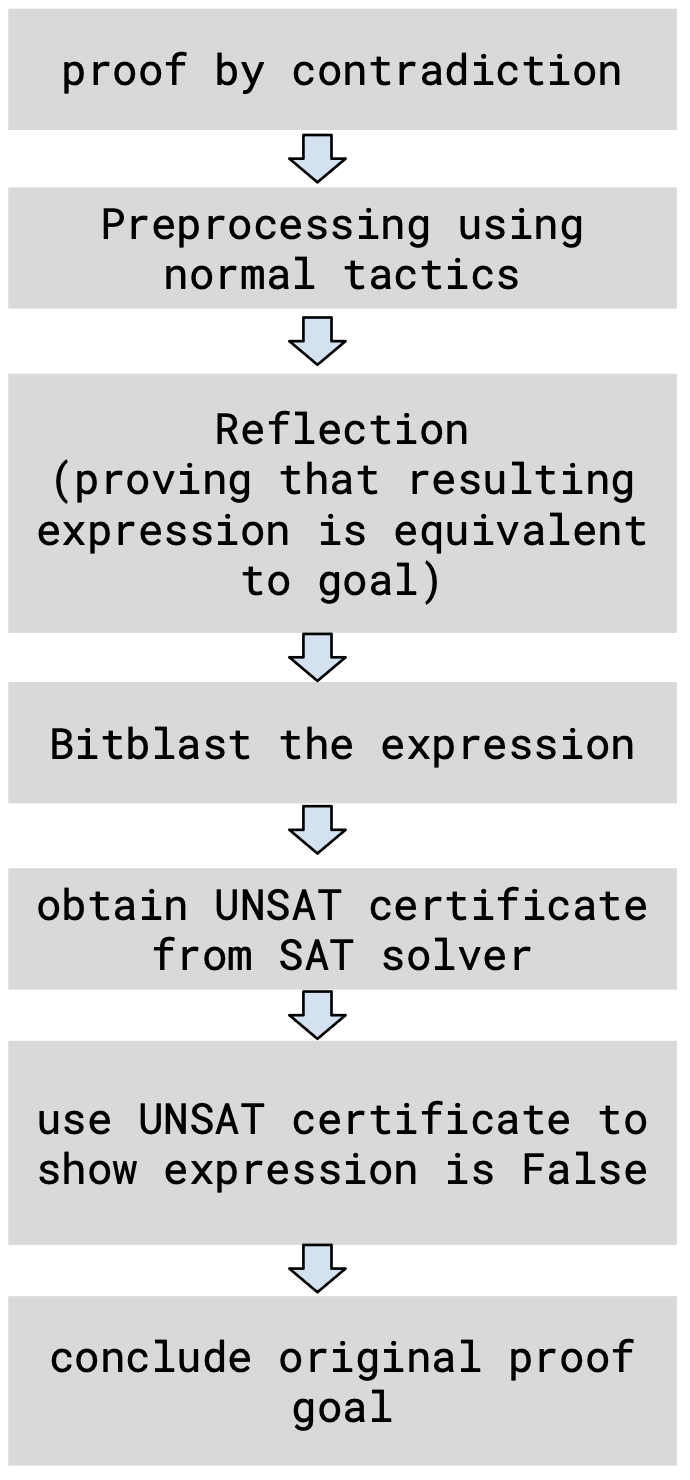
\includegraphics[scale=0.37]{thesis/bv_decide.png}
 
  \caption{Bv\_decide procedure flow}
  \label{fig:your-label}
\end{figure}

\textit{Contradiction Derivation}: Bv\_decide transforms the original goal into a contradiction form and starts a proof by contradiction. This allows for proving unsatisfiability of the contrary proof goal instead of forwards proving the original proof goal. 

\textit{Preprocessing}: Then bv\_decide normalizes and simplifies the goal by rewriting bit-vector expressions. It leverages rewrite rules inspired by the Bitwuzla SMT solver to perform these simplifications. Additionally, it performs and-flattening, which examines all currently available hypotheses, splits any conjunctions into individual hypotheses, and repeatedly applies rewriting across hypotheses until a fixed point is reached.

\textit{Reflection}: Proof by reflection is then used to show that transforming a bit-vector goal into a form where bit-vector operations are reified using additional Lean data structures preserves semantic equivalence. Wrapping bit-vector operations in these constructs enables easier processing in subsequent steps. The reflection proof guarantees that any proposition involving the enriched Lean representation is logically equivalent to a corresponding proposition about bit-vectors alone.

\textit{Bitblasting}: A verified bitblasting algorithm is then used to convert the reified bit-vector expression into an And-Inverter Graph (AIG), a data structure commonly used to efficiently represent Boolean circuits. This transformation reduces the high-level bit-vector goal to a low-level Boolean SAT problem. Finally, the AIG is translated into a conjunctive normal form (CNF) formula.

\textit{External Solving}: The CNF formula is sent to an external SMT solver, which attempts to produce an UNSAT certificate demonstrating that the formula is unsatisfiable. If the formula is satisfiable instead, the solver returns a counterexample.

\textit{Certificate Reflection}: If the SMT solver proves the formula is unsatisfiable (UNSAT), it returns an UNSAT certificate, which is imported back into Lean. The certificate is then checked within Lean ensuring that the unsatisfiability result is trustworthy and fully formalized.

\textit{Proof Construction}: Finally, the verified UNSAT certificate is used to construct a formal Lean proof of the original goal. Since the conjunction of the assumptions and the negation of the goal has been shown to be unsatisfiable, it logically follows that the original goal must be true. All previous proof steps are composed to conclude the overall proof.

Invoking the whole bv\_decide procedure to solve bit vector proof goals in Lean is illustrated below.
\begin{lstlisting} [language=python, caption= Discharging bit vector proof goal using bv\_decide]
theorem bv_add_comm {w : Nat} (a b : BitVec w) : BitVec.add a b 
    = BitVec.add b a := by
  bv_decide

theorem bv_mul_distr {w : Nat} (a b c : BitVec w) : 
  BitVec.mul a (BitVec.add b c) 
    = BitVec.add (BitVec.mul a b) (BitVec.mul a c) := by
  bv_decide
\end{lstlisting}

At the time of this thesis, bv\_decide handles a significant fragment of bit-vector logic and operations on bit vectors. However, it exhibits limitations in expressions that involve conversions between natural numbers and bit vectors, as natural numbers are unbounded in Lean and bit blasting requires a fixed-bounded width. Bv\_decide treats unknown variables or nonfixed-width bit vectors as undefined variables, however, yet attempts to resolve the goal within this abstraction. If the tactic fails to produce a proof, it returns a counterexample indicating which terms were treated as variables, providing insights into why the proof attempt failed(Listing 2.5). This interactive feedback exemplifies Lean's strength as an interactive theorem prover that leverages human-computer interaction to prove complex goals. This approach contrasts with common SMT solvers, which are proficient in solving fixed-width bit vector problems but do not support tools for interaction with the developer.


\begin{lstlisting} [language=python, caption= Example feedback by bv\_decide when trying to proof arbitrary-width bit vector theorem]
The prover found a potentially spurious counterexample:
- It abstracted the following unsupported expressions
as opaque variables: -- here the abstracted variables
will be listed.}
\end{lstlisting}





To enhance the performance of the bv\_decide procedure and avoid redundant calls to the external SMT solver, bv\_decide employs a caching mechanism for previously verified results. Additionally, the bv\_decide tactic has several configuration options to adapt its behavior to the specific structure of the proof goal e.g time-bound parameter that limits the solver execution. 

Invoking bv\_normalize instead of bv\_decide runs only the normalization step of bv\_decide  and is used in proof goals where automated algebraic normalization and simplification of bit vector terms without invoking the SAT solver suffices. If the proof goal is solved by bv\_normalize the SMT solver invocation and bit-blasting are skipped by bv\_decide. 
\section{Verified Instruction Selection and Peephole Optimizations } 
\subsection{Peephole Optimizations} 

\section{Llvm ir , Riscv and their semantics} 


\noindent
\begin{minipage}{0.6\textwidth}
\begin{lstlisting}[language=Python, caption=unoptimized]
int check(int x) {						        
	if (x == 0) return 0; 					
    else return x;
    def BitVec (w : Nat) := { n : Nat // n < 2^w }
}
\end{lstlisting}
\end{minipage}
\hfill
\begin{minipage}{0.45\textwidth}
\begin{lstlisting}[language=C, caption= optimzed assembly]
check: 
    mov r0, r0
}
\end{lstlisting}
\end{minipage}


\section {Semanctics}


\chapter{Extracting Instruction Selection Patterns}




\chapter{Related Work }
This section presents work in the broader area of verified compilation as well as verification projects specifically targeting the LLVM ecosystem. We present contributions from validating single optimization passes to fully end to-end verified compilerse. In addition, we discuss previous work on the formalization of LLVM IR and ISA semantics as well as compiler testing.

\textbf{Verified Compilation}
In the past various efforts have been performed to apply formal methods to the compiler design space. We could identify two prominent approaches to exist: The first approach focuses on the implementation of new fully verified compilation infrastructures where the correctness of the compiler component is verified once and for all. This approach usually requires large manual proof effort and provides limited optimization. The second approach verifies existing mainstream compiler components through the use of translation validation techniques. Translation validation refers to certifying that an execution stage of a compiler is correct by verifying the semantic equivalence between the input and output of the individual stage.  

A prominent example of the first approach is CompCert [ Leroy et al.] an optimizing compiler for a large subset of the C programming language, ".. which is formally verified, using machine-assisted mathematical proofs, to guarantee the absence of compiler bugs."  CompCert compiles C programs into machine code for various processor targets, including RISC-V, and provides formal correctness guarantees for its compilation process. The compiler is implemented in the RCoq proof assistant and goes through 8 IR's and 15 compilation passes before outputting assembly code. Optimizations in CompCert is limited by the manual effort to provide the correct proof and constantly adapt the compiler to support the new optimization pattern without breaking existing proofs. 

For verification, CompCert based their ISA semantics on manual translations from the ISA specification into RCoq. There is no indication that CompCert integrates external machine-checked ISA models, such as those generated from the Sail language. In this regard, our work provides correctness proofs that our RISC-V semantics correspond to the machine-formalized semantics accepted by RISC-V International. Due to its limited optimization support, CompCert has been relegated to specialized contexts where full correctness is safety-critical. In contrast, Alive is a project that has gained wide spread acceptance within the LLVM ecosystem and showcases that verification and automation within the mainstream compiler design space is possible, useable and accepted by compiler developers. Alive provides a tool to automatically verify the correctness of LLVM IR optimizations. It checks the input and output for refinement using an SMT solver for verification. Alive can miss bugs in certain circumstances as it is a bounded translation validation tool e.g. sets an upper bound to unfolding loops. Bugs that would be exposed by continuously unfolding are missed. Therefore as stated in their paper, "there are certain circumstances in which it misses bugs". 

\textbf{Verified Peephole Optimization}
Assembly-level peephole transformations are common in compilers and are known to be particularly bug-prone. [quote peek paper] Various efforts have been made to verify and implement local rewrite patterns and ensure their correctness. One effort is Peek, a framework for expressing, verifying, and executing machine code transformations for x86 within CompCert. However, Peek requires the peephole rewrite patterns to be linear and adjacent. Contrary to the peephole hole rewriter in Lean-MLIR, which can optimize across non-linear instruction sequences interleaved with unrelated instructions. Peek explicitly models side effects and includes a memory-related rewrites. Similar to our work, Peek reasons that applying locally semantics-preserving rewrites preserves the global meaning of the program.

Additional work on verifying peephole optimizations was conducted by the Lean-MLIR project [7], which is discussed in detail in a dedicated section. In particular, Lean-MLIR formalized and verified several of the peephole rewrites used in InstCombine, a widely-used LLVM IR optimization pass. Alive also provides a verification tool for LLVM's peephole optimizations while AliveInLean is a reimplementation of the project in Lean. There have been verification efforts for peephole optimizations in other programing languages.  [] developed a verification tool for rewrites in Halide. 
[https://arxiv.org/pdf/2407.03685,
https://coqpl.cs.washington.edu/wp-content/uploads/2014/12/peek.pdf
]

\textbf{Lean-MLIR}
We mention lean-MLIR in this section to highlight the related projects built with Lean-MLIR, while details of the framework itself are covered in Chapter 3. Tobias et Al. published a paper on “Verifying Peephole Rewrites in SSA Compiler IRs” introducing Lean-MLIR framework and derived projects from it. The Lean-MLIR framework was used to reimplement and formally verify 93 test cases from Alive2, which demonstrated the use of Lean-MLIR to real world compiler optimization patterns. Using Lean-MLIR to verify the test cases used in Alive exposed xy bugs.  At the time of this thesis, Lean-MLIR had been used to formulate and verify rewrites within single IR's such as LLVM IR. However, Lean-MLIR has not been extended to support cross-dialect transformations or used to model hardware-level assembly IR's. This gave the potential to further develop the work in the direction of dialect lowerings and low-level language optimizations. Inspired by this we extend the application of Lean-MLIR and its verification methodology across multiple layers of a compiler pipeline, by adding a instruction selection pass and machine-level transformations. Other efforts on Lean-MLIR have formalized various dialects, including one for fully homomorphic encryption. Additionally, the authors of Lean-MLIR have conducted research on effective automation for bit-vector reasoning, which is essential for discharging proof goals in programs that use bit vectors as their semantic model.

\textbf{Formal Semantics of LLVM IR}
The formalization of LLVM IR semantics has been at focus of several research. Verification tools like Alive have found bugs in LLVM that stem from simple logical implementation errors. Besides the typical logical implementation errors, there are bugs caused by underspecification of the LLVM IR semantics which leads to different interpretations of certain instructions in a given context. To build verification tools and distinguish miscompilations from correct compilations,  consensus on the specification of LLVM IR is needed. The intended semantics of LLVM IR are documented online in the reference manual but are not exhaustive and do not provide a  rigourous mathematically formalization of the semantics. Given the size and high activity of the LLVM community, there exist a lack of coordination on the accepted semantics of LLVM IR, and any discrepancy in how semantics are interpreted leads to subtle bugs, as history has shown [Alive paper]. Vellvm is one effort to formalize the semantics of LLVM IR and provides a framework for reasoning about LLVM IR programs. Unlike our work, Vellvm is implemented in the Coq theorem prover and uses a definition of refinement that differs from the one used in this thesis.  We also do not adopt the semantics formalized in Vellvm because they do not satisfy the monotonicity property that we believe should hold. Similar to our work, Vellvm does not support all forms of UB e.g. they fix all undef values to a zero initializer. Besides Vellvm, the authors of Alive provide a formalization of LLVM IR in their paper. Alive interacted with the LLVM community to iterate over underspecified parts and reached consensus on how to fix discrepancies in the LLVM IR semantics—e.g., how the select instruction interacts with poison values. This work performed by Alive is relevant to our own, since our semantic model provided by Lean-MLIR is close to the Alive formalization except for the mentioned UB. The semantics of UB have been explored in [taming UB paper] and proposed changes adapted by LLVM.  For any formal methods efforts in the LLVM ecosystem, formalizations of LLVM IR are crucial and therefore we mention this work in this section. 

[taming udef by hjohn regehr, vellvm, alive ]
[https://dl.acm.org/doi/pdf/10.1145/2103621.2103709]


\textbf{Compiler testing and fuzzing}
Besides formal verification, which provides strong correctness guarantees and can prove the absence of bugs, as demonstrated in CompCert, testing and fuzzing tools have been highly effective in identifying compiler bugs. Several bugs in the optimizers of commercial compilers, including LLVM, have been discovered by tools such as those described in [citation].

[to do: add further work on this]
[to do: formally show where Vellvm's semantics fail this].
[to do: extend with a more in depth disccusion on work on the semantics]
[https://dl.acm.org/doi/pdf/10.1145/2103621.2103709]
[TO DO check vellvm refinement statement]


\chapter{Typography}


\section{Punctuation}

\begin{Rule}
  Use opening (`) and closing (') quotation marks correctly.
\end{Rule}

In \LaTeX, the closing quotation mark is typed like a normal
apostrophe, while the opening quotation mark is typed using the French
\emph{accent grave} on your keyboard (the \emph{accent grave} is the
one going down, as in \emph{frère}).

Note that any punctuation that \emph{semantically} follows quoted
speech goes inside the quotes in American English, but outside in
Britain.  Also, Americans use double quotes first.  Oppose
\begin{quote}
  ``Using `lasers,' we punch a hole in \ldots\ the Ozone Layer,''
  Dr.\ Evil said.
\end{quote}
to
\begin{quote}
  `Using ``lasers'', we punch a hole in \ldots\ the Ozone Layer',
  Dr.\ Evil said.
\end{quote}

\begin{Rule}
  Use hyphens (-), en-dashes (--) and em-dashes (---) correctly.
\end{Rule}

A hyphen is only used in words like `well-known', `$3$-colorable'
etc., or to separate words that continue in the next line (which is
known as hyphenation).  It is entered as a single ASCII hyphen
character (\texttt{-}).

To denote ranges of numbers, chapters, etc., use an en-dash (entered
as two ASCII hyphens \texttt{--}) with no spaces on either side.  For
example, using Equations (1)--(3), we see\ldots

As the equivalent of the German \emph{Gedankenstrich}, use an en-dash
with spaces on both sides -- in the title of Section \ref{sec:list},
it would be wrong to use a hyphen instead of the dash. (Some English
authors use the even longer emdash (---) instead, which is typed as
three subsequent hyphens in \LaTeX. This emdash is used without spaces
around it---like so.)


\section{Spacing}

\begin{Rule}
  \label{rule:no-manual-spacing}
  Do not add spacing manually.
\end{Rule}

You should never use the commands \lstinline-\\- (except within
tabulars and arrays), \lstinline[showspaces=true]-\ - (except to
prevent a sentence-ending space after Dr.\ and such),
\lstinline-\vspace-, \lstinline-\hspace-, etc.  The choices programmed
into \LaTeX{} and this style should cover almost all cases.  Doing it
manually quickly leads to inconsistent spacing, which looks terrible.
Note that this list of commands is by no means conclusive.

\begin{Rule}
  Judiciously insert spacing in maths where it helps.
\end{Rule}

This directly contradicts Rule~\ref{rule:no-manual-spacing}, but in
some cases \TeX{} fails to correctly decide how much spacing is
required.  For example, consider
\begin{displaymath}
  f(a,b) = f(a+b, a-b).
\end{displaymath}
In such cases, inserting a thin math space \lstinline-\,- greatly
increases readability:
\begin{displaymath}
  f(a,b) = f(a+b,\, a-b).
\end{displaymath}

Along similar lines, there are variations of some symbols with
different spacing.  For example, Lagrange's Theorem states that
\(\abs{G}=[G:H]\abs{H}\), but the proof uses a bijection \(f\colon
aH\to bH\).  (Note how the first colon is symmetrically spaced, but
the second is not.)

\begin{Rule}
  Learn when to use \lstinline[showspaces=true]-\ - and
  \lstinline-\@-.
\end{Rule}

Unless you use `french spacing', the space at the end of a sentence is
slightly larger than the normal interword space.

The rule used by \TeX{} is that any space following a period,
exclamation mark or question mark is sentence-ending, except for
periods preceded by an upper-case letter.  Inserting \lstinline-\-
before a space turns it into an interword space, and inserting
\lstinline-\@- before a period makes it sentence-ending.  This means
you should write
\begin{lstlisting}
Prof.\ Dr.\ A. Steger is a member of CADMO\@.
If you want to write a thesis with her, you
should use this template.
\end{lstlisting}
which turns into
\begin{quote}
  Prof.\ Dr.\ A. Steger is a member of CADMO\@.  If you want to write
  a thesis with her, you should use this template.
\end{quote}
The effect becomes more dramatic in lines that are stretched slightly
during justification:
\begin{quote}
  \parbox{\linewidth}{\hbox to \linewidth{%
      Prof.\ Dr.\ A. Steger is a member of CADMO\@.  If you}}
\end{quote}

\begin{Rule}
  Place a non-breaking space (\lstinline-~-) right before references.
\end{Rule}

This is actually a slight simplification of the real rule, which
should invoke common sense.  Place non-breaking spaces where a line
break would look `funny' because it occurs right in the middle of a
construction, especially between a reference type (Chapter) and its
number.


\section{Choice of `fonts'}

Professional typography distinguishes many font attributes, such as
family, size, shape, and weight.  The choice for sectional divisions
and layout elements has been made, but you will still occasionally
want to switch to something else to get the reader's attention.  The
most important rule is very simple.

\begin{Rule}
  When emphasising a short bit of text, use \lstinline-\emph-.
\end{Rule}

In particular, \emph{never} use bold text (\lstinline-\textbf-).
Italics (or Roman type if used within italics) avoids distracting the
eye with the huge blobs of ink in the middle of the text that bold
text so quickly introduces.

Occasionally you will need more notation, for example, a consistent
typeface used to identify algorithms.

\begin{Rule}
  Vary one attribute at a time.
\end{Rule}

For example, for \textsc{WeirdSort} we only changed the shape to small
caps.  Changing two attributes, say, to bold small caps would be
excessive (\LaTeX{} does not even have this particular variation).
The same holds for mathematical notation: the reader can easily
distinguish \(g_n\), \(G(x)\), \(\mathcal{G}\) and \(\mathsf{G}\).

\begin{Rule}
  Never underline or uppercase.
\end{Rule}

No exceptions to this one, unless you are writing your thesis on a
typewriter.  Manually.  Uphill both ways.  In a blizzard.


\section{Displayed equations}

\begin{Rule}
  Insert paragraph breaks \emph{after} displays only where they
  belong.  Never insert paragraph breaks \emph{before} displays.
\end{Rule}

\LaTeX{} translates sequences of more than one linebreak (i.e., what
looks like an empty line in the source code) into a paragraph break in
almost all contexts.  This also happens before and after displays,
where extra spacing is inserted to give a visual indication of the
structure.  Adding a blank line in these places may look nice in the
sources, but compare the resulting display

\begin{displaymath}
  a = b
\end{displaymath}

to the following:
\begin{displaymath}
  a = b
\end{displaymath}
The first display is surrounded by blank lines, but the second is not.
It is bad style to start a paragraph with a display (you should always
tell the reader what the display means first), so the rule follows.

\begin{Rule}
  Never use \lstinline-eqnarray-.
\end{Rule}

It is at the root of most ill-spaced multiline displays.  The
\package{amsmath} package provides better alternatives, such as the
\lstinline-align- family
\begin{align*}
  f(x) &= \sin x, \\
  g(x) &= \cos x,
\end{align*}
and \lstinline-multline- which copes with excessively long equations:
\begin{multline*}
  \def\P{\mathrm P}
  \P\bigl[X_{t_0} \in (z_0, z_0+dz_0],\ldots, X_{t_n}\in(z_n,z_n+dz_n]\bigr]
  \\= \nu(dz_0) K_{t_1}(z_0,dz_1) K_{t_2-t_1}(z_1,dz_2)\cdots
  K_{t_n-t_{n-1}}(z_{n-1},dz_n).
\end{multline*}


\section{Floats}

By default this style provides floating environments for tables and
figures.  The general structure should be as follows:
\begin{lstlisting}
\begin{figure}
  \centering
  % content goes here
  \caption{A short caption}
  \label{some-short-label}
\end{figure}
\end{lstlisting}
Note that the label must follow the caption, otherwise the label will
refer to the surrounding section instead.  Also note that figures
should be captioned at the bottom, and tables at the top.

The whole point of floats is that they, well, \emph{float} to a place
where they fit without interrupting the text body.  This is a frequent
source of confusion and changes; please leave it as is.

\begin{Rule}
  Do not restrict float movement to only `here'
  \textnormal{(\lstinline-h-)}.
\end{Rule}

If you are still tempted, you should avoid the float altogether and
just show the figure or table inline, similar to a displayed equation.

%%% Local Variables:
%%% mode: latex
%%% TeX-master: "thesis"
%%% End:

\chapter{Example Chapter}

Dummy text.

\section{Example Section}

Dummy text.

\subsection{Example Subsection}

Dummy text.

\subsubsection{Example Subsubsection}

Dummy text.

\paragraph{Example Paragraph}

Dummy text.

\subparagraph{Example Subparagraph}

Dummy text.


\appendix

\chapter{Dummy Appendix}

You can defer lengthy calculations that would otherwise only interrupt
the flow of your thesis to an appendix.


\backmatter

\bibliographystyle{plain}
\bibliography{refs}

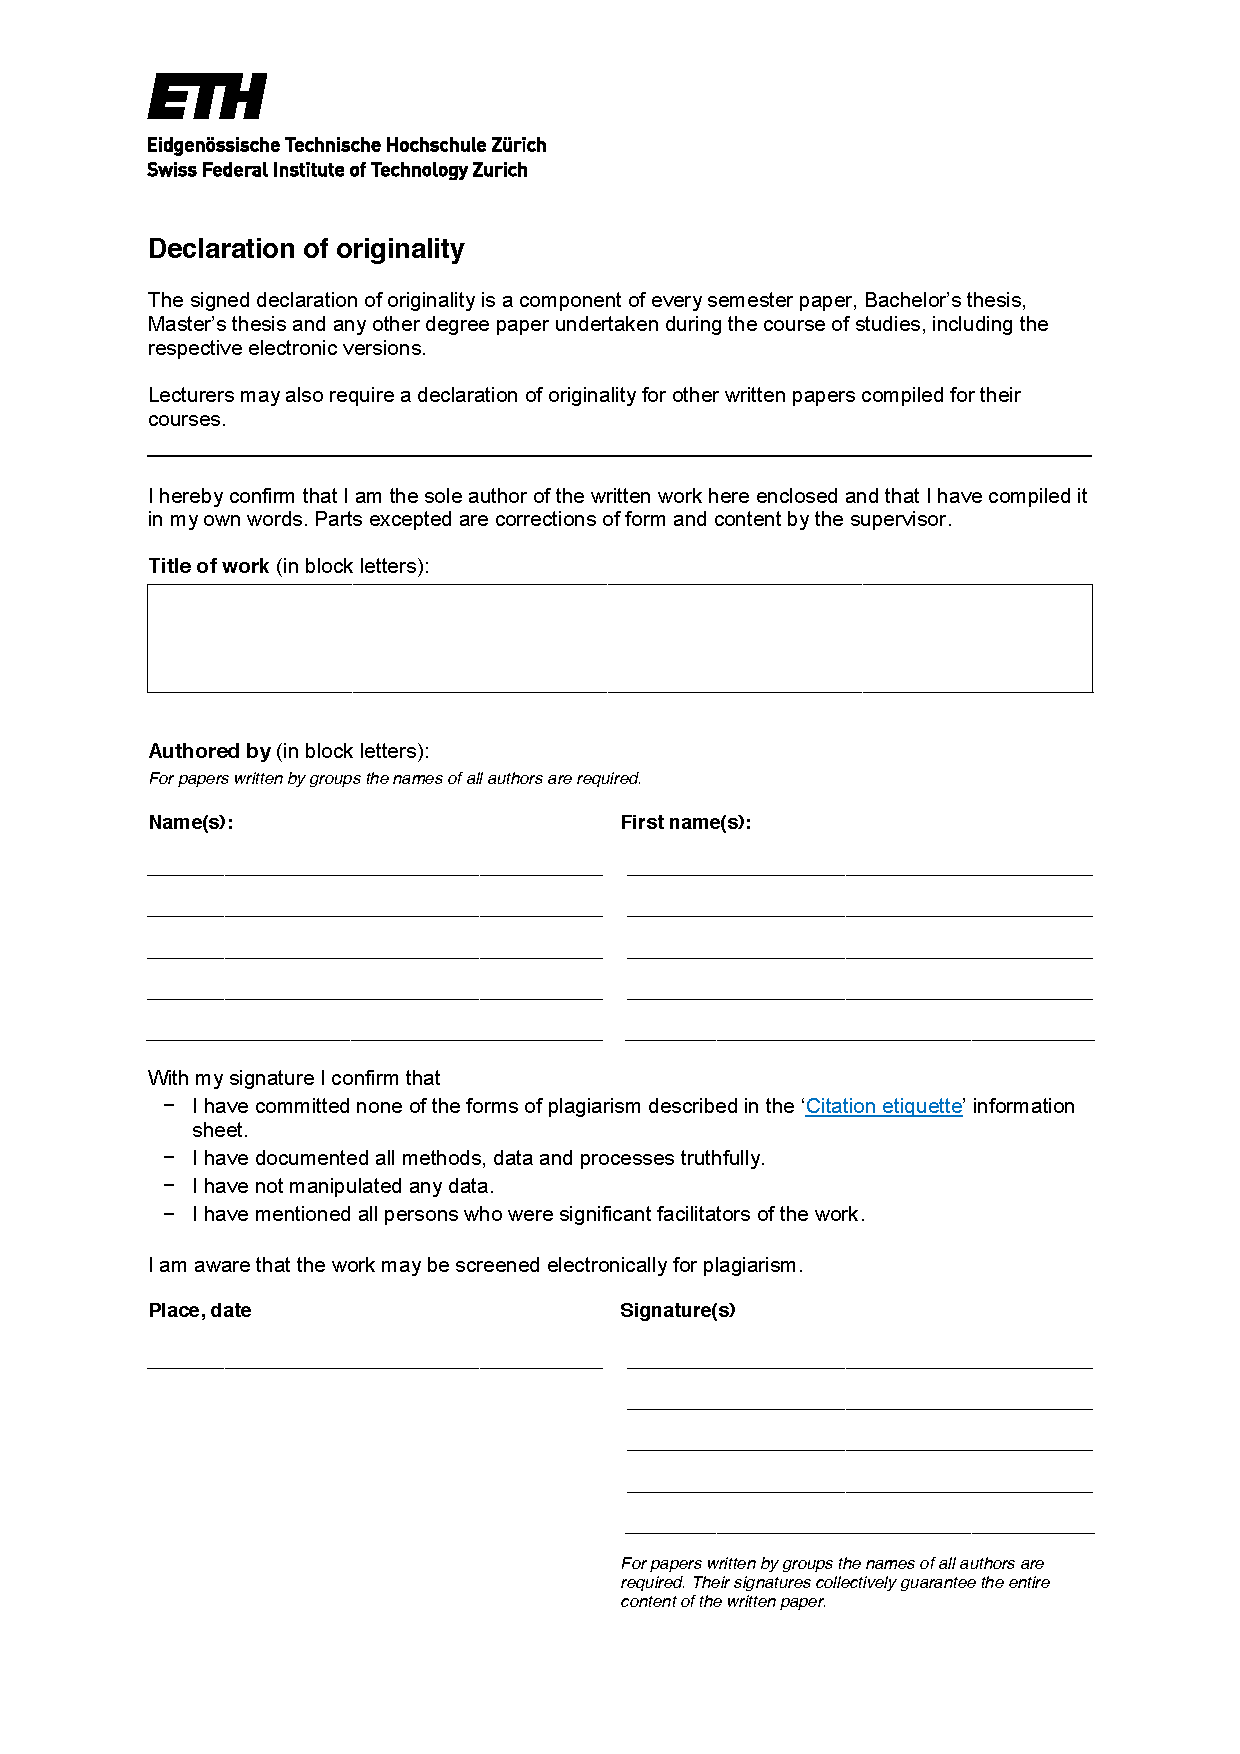
\includepdf[pages={-}]{declaration-originality.pdf}

\end{document}
